\chapter{Accelerated Discovery of High-Refractive-Index Polyimides}

Polyimides have attracted much attention due to their exceptional thermal stability and ease of processability. Further, polyimides possess mechanical stability, good flexibility, flame resistance, radiation resistance and low dielectric constant, thus holding great promises for various applications.  However, these polymers have low refractive index (RI) values which limit their use in optical and optoelectronic applications. In this study, we present a computational approach to discover novel high RI polyimides (PI). We use an RI prediction model, developed in our previous work, to calculate the RI values of large candidate library of PIs, created from building blocks provided by our experimental collaborators. To accelerate the development process and effectively screen the relevant high RI PIs, we cast the RI model into \chemhtps: a high-throughput screening, materials informatics, and rational design framework software developed in our group. We prove that \chemhtps\ is promising for rapidly identifying PIs with exceptionally high RI values. We explore various paths that introduce highly polarizable moieties into PI backbones to increase RI. We also identify monomer building blocks within PIs that are prevalent in high RI PIs, and discover building block combinations that result in the same. Additionally, we provide insights into the relationship between the structure and the RI values of polyimides, thus allowing us to target most promising candidates. We thank Prof. Cheng for providing us with building blocks and generation rules for synthetic feasibility. We acknowledge Sai Prasad Ganesh for his contributions in this work. He contributed to understanding the dependence of the polarizability on the geometry of molecules.  


\section{Introduction}
\label{sec:introduction5}

%Addressing the need for discovery of high RI polymers
Organic small molecules, oligomers, and polymers are emerging materials that feature many attractive properties compared to conventional inorganic materials. Devices made out of organic polymers are generally flexible, mechanically stable on impact, light-weight, and inexpensive to produce. This has led to increased efforts in utilizing these compounds in many different application domains, including optic and optoelectronic devices such as organic light-emitting diodes \cite{ThejoKalyani2012}, complementary metal oxide semiconductor \cite{Nakagawa2010},  photovoltaics \cite{Hachmann2011}, field-effect transistors \cite{Sirringhaus2009}, displays, and image sensors \cite{Angione2011}, in which they can be introduced \insitu\ as microlenses, waveguides, microresonators, interferometers, anti-reflective coatings, optical adhesives, and substrates. However, most of these applications require materials with a refractive index (RI) greater than 1.7 or larger, while typical carbon-based polymers only exhibit values in the range of 1.3-1.5 \cite{Liu2009}. This provides an incentive to discover or design new high-refractive index polymers (HRIPs) for the aforementioned applications. As the properties of organic polymers can be tailored by controlling their molecular structure, they are a prime example for a rational design target.

%Polyimides properties leading to a promising candidate for optoelectronic devices
In recent years, polyimides (PIs) have been shown to have favorable electronic and mechanical properties that could form potential HRIP candidates. Despite showing inherently low RI values leading to a lack of present applicability, PIs have other attractive properties \citep{Mathews2007,Chang2006}.  
PIs are strong potential candidates due to their exceptional thermal stability, and ease of processability \citep{Duesselberg2011,Liu2007a,Higashihara2015}. These properties are complemented by their favorable mechanical stability, flexibility, flame resistance, radiation resistance and their sufficiently high molecular polarizability: properties which would allow for potential use in optoelectronics \citep{Mittal2013,Barikani2000}.

%PI’s poor optical properties, especially RI, limiting its use in these devices
As previously mentioned, the optical properties of PIs are significantly inferior compared to conventional metal oxides currently used in optical and optoelectronic devices \citep{Butnaru2013,Liu2009}. However, PI optical properties can be improved upon by several methods \citep{Fukuzaki2010,Liu2008b,Sydlik2011,Terraza2008,Carter2001}. One such technique is to control the chemical structure of PIs to allow for precise tuning of optical properties, in particular to increase their RI values \citep{Liu2007a,Terraza2008,Yu1995,You2008}. In our study, we present a computational approach to study the RI of PIs and explore techniques that introduce highly polarizable moieties into polyimides framework to create a new class of high RI PIs. 

%Although, addition of some highly polarizable moieties might result in the discoloration of the PI material \cite{Barikani2000}. (Need more information on this, or remove it)

%Recent empirical approaches in increasing PI RI values by introducing different functional groups
Typically, HRIPs exist in the form of aromatic polyamides, and aromatic heterocyclic ring polymers, and certain conjugated aromatic polymers. However, these HRIPs struggle when it comes to optical implementation due to their large optical dispersion and large birefringence. The large birefringence is caused due to their aromatic, and conjugated pi-electron structures, which leads to poor transparency and coloration. The addition of highly polarizable moieties, which do not have significant pi-electron conjugation, can aid in increasing the RI of polymers. For example, small aromatic rings, halogen atoms, metals and particularly sulfur atoms have shown to be promising for this purpose \citep{Tsai2016,Kobayashi1998,Liu2007a,Sawada1998}. Previous experimental studies have demonstrated the ability of sulfur infused PIs to overcome potential unfavorable properties. In particular, high thermal stability, a low birefringence, an optical transparency in the visible light region, and high RI values have been demonstrated. In 2007, Ueda \textit{et. al.} developed PI films which were shown to have high RI values, but had unfavorably high birefringence in the range of 0.012 \cite{Liu2007b}. However, in recent years, experimental work has shown improvement in terms of birefringence and RI, with RI in the range of 1.76 and birefringence of 0.009 attained in particular, due to the high sulfur content of the PIs \cite{Yeo2015}. These encouraging results have led to our study being primarily concerned with sulfur incorporated PIs, and in doing so, generate a new class of HRIPs that does away with the technical limits of existing HRIPs.

%Number of possible options to create PI with potentially high RI values. However, there is limitation in what empirical studies could attain. With some input from empirical expertise, the computational studies could get the right direction to focus in the large chemical space.
Most of the PIs developed for high RI applications are based on the intuition of empirical observations. Therefore, there is a high possibility that there are potential HRIP candidates that are not studied experimentally simply because there are too many possible candidates to be feasibly studied. This motivation has led to our approach in generating a large library of promising PI candidates created by our molecular library generator. The library generator operates based on combinatorial linking, which could possibly to lead to an astronomical number of candidates beyond the scope of affordable computational studies. To counteract this, we narrowed the candidates generated from the library based on keen observations from past research and generation rules based on the input provided from our experimental collaborators. We created our PI library by casting these rules into the molecular library generator. We used our RI prediction model to evaluate the RI values of generated PI candidates \cite{Afzal2018a}.

%Accelerating the process of PI by using the RI protocol and in-house virtual high throughput screening framework. 
To facilitate RI evaluation of our large pool of candidates in a timely manner we use our virtual high-throughput screening framework, \chemhtps\ \cite{Afzal2018c}., that draws inspiration from The Harvard Clean Energy Project, which was successfully screened millions of organic molecules for photovoltaic applications \citep{Hachmann2011,Hachmann2014,Olivares-Amaya2011}. \chemhtps\ creates inputs, executes and monitors the calculations, parses and assesses the results, extracts and post-processes the information of interest, inserts the key outcomes into the project database, and archives all other data. Using this \insilico\ methodology we created a large number of novel PI candidates and characterized these candidates at a fraction of the time and cost of traditional studies.

\section{Methods}
\label{sec:methods5}
%1.	Refer the protocol to determine the polarizability and RI of polymers from previous paper
In our previous work, we developed a model for the prediction of RI of polymers, which was validated against experimental RI values of 112 non-conjugated polymers \cite{Afzal2018a}.  The RI prediction model is based on a synergistic combination of \textit{first-principles} quantum chemistry calculations and data modeling. In this scheme, we calculate RI values using the Lorentz-Lorenz equation, which involves two critical parameters, the number density and the polarizability. We calculate the former using van der Waals volume and packing factor of the polymer, while for the polarizability calculations, we use \firstprinciples. 

%2.	Describing tools for automating the framework of RI calculation of polymers using different method
We developed a library of PIs using our molecular library generator, \chemlg\ \cite{Afzal2018b}. The library is based on 29 building blocks and bonding rules (see Fig. \ref{fig:Building_blocks}, which were selected based on the suggestions provided by our experimental collaborator, Cheng's group. Based on these generation rules, we created about 50 thousand and 230 thousand possible structures for $R_1$ and $R_2$, respectively. We saved the structures in the form of SMILES string along with a code which contains the information on the list of building blocks and connections that were used to make a particular structure. We subsequently used \chemhtps\ to screen the PI candidates to evaluate their RI values, and collected the data in our project database. 
%TODO - more information about the database or the supplementary information.

For each $R_1$ and $R_2$ SMILES, we generated fifty different 3D conformations using OpenBabel software \cite{OBoyle2011}. We selected the lowest energy conformation for each structure and further optimized the geometry using the universal force field (UFF) \cite{Rappe1992} as implemented in the OpenBabel software. We use a packing factor of 0.75 to calculate the number density of PIs, as previous experimental studies have shown that PIs typically have a packing factor of 0.75 \cite{Privalko1997}. 
%We do not use the previously developed data model for calculating the packing factor of PIs. This is because the PIs studied in this work are structurally different than the polymers that were used to build the data model. 
We calculated the van der Waals volumes using Slonimskii's method detailed in Ref.\ \cite{Slonimskii1970}. For the polarizability calculations, we use an all-electron, restricted DFT method with the PBE0 hybrid functional \cite{Adamo1999} in combination with the double-$\zeta$ quality def2-DZVP basis set by the Karlsruhe group \cite{Weigend2005}. We include Grimme's D3 correction \cite{Grimme2010} to account for dispersion interaction. We carried out all the quantum computations using the ORCA 3.0.2 quantum chemistry package \cite{Neese2012}. 


\begin{figure}[htbp] 
	\centering
	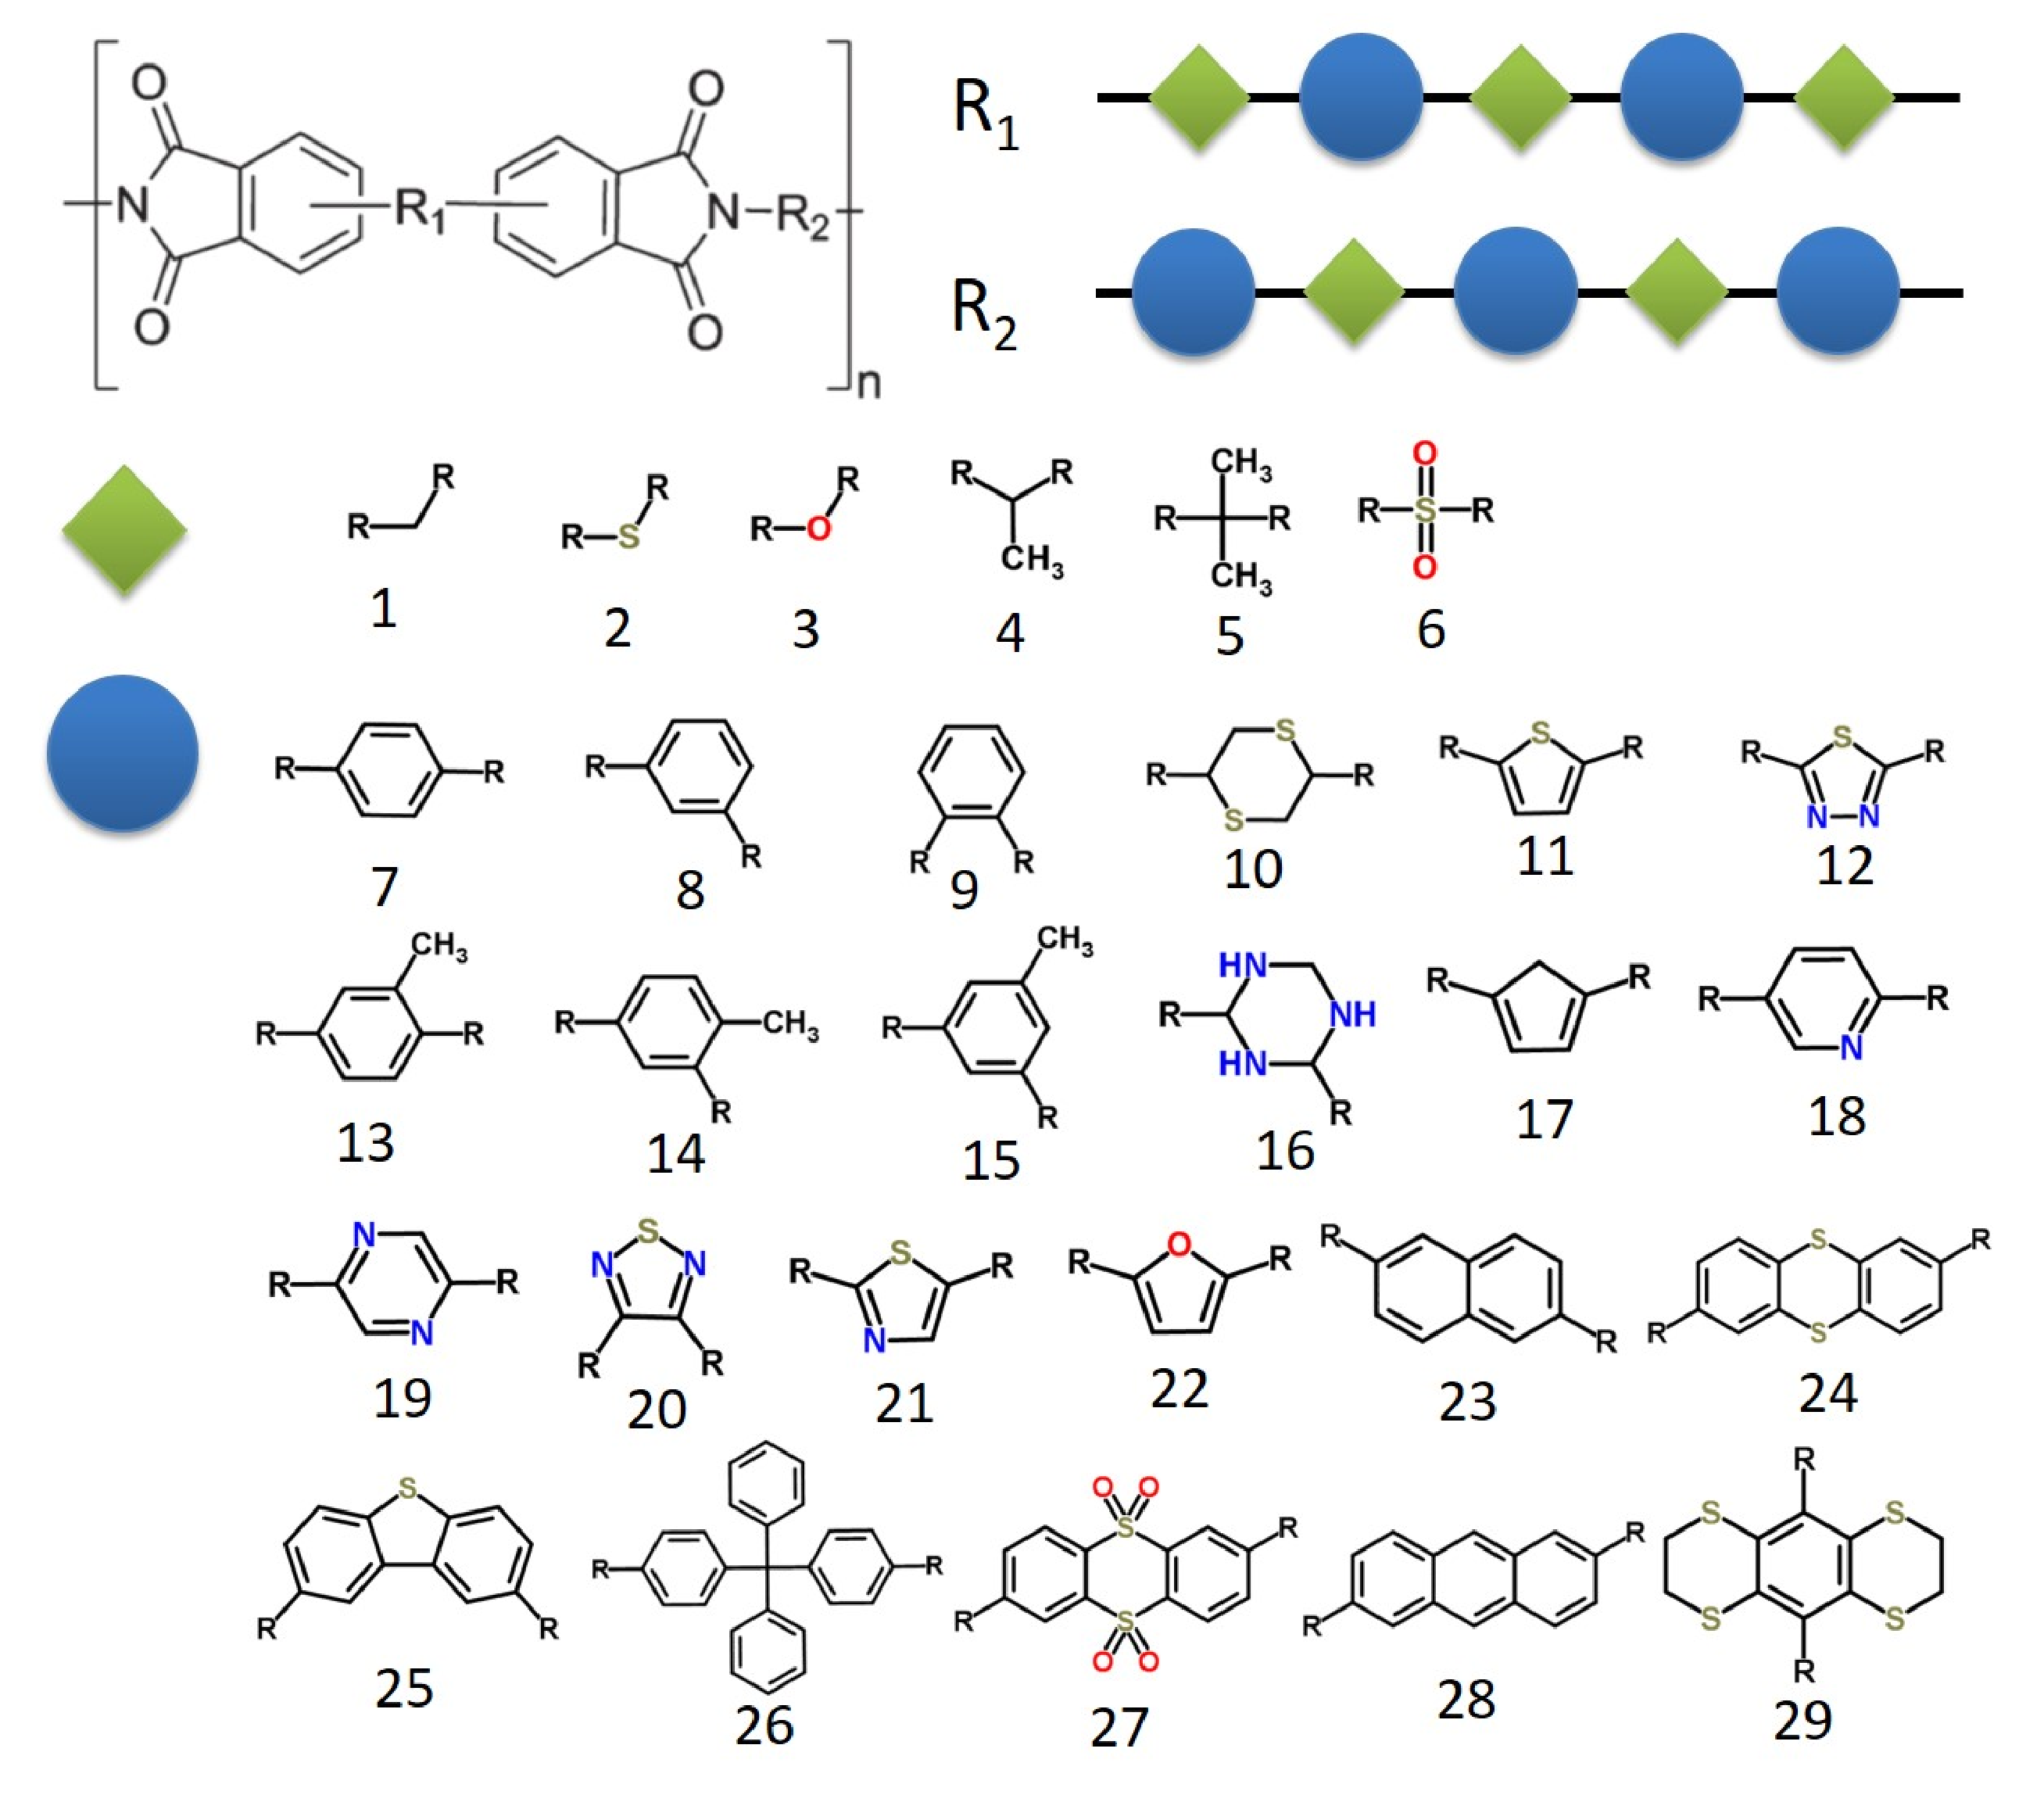
\includegraphics[width=0.744\textwidth]{Chapter-5/Figures/Building_blocks.eps}
	\caption{Building blocks used to create the library of PIs.} 
	\label{fig:Building_blocks} 
\end{figure} 

%3.	Describe the approach considered in understanding the structure-property relationships. 
In addition to identifying the best candidates from our high-throughput screening studies, we further analyze the collected data to understand structure-property relations. By applying Z-score analysis, we identify the building blocks that contribute the most to the RI values. We compute the Z-score ($Z_i$) of the candidates by
\[
Z_i=\frac{k-n\frac{K}{N} }{\sigma},\ \sigma=\left [ \frac{nK}{N}\times \left ( \frac{N-K}{N} \right )\times \left ( \frac{N-n}{N-1} \right )\right ]^{\frac{1}{2}}
\]
where $N$ is the total number of molecules, $n$ is the subset of molecules that are considered, $K$ number of occurrences of building block $i$ in $N$ molecules and the $k$ is the occurrences of building block $i$ in $n$ subset. We perform similar calculations to calculate the Z-score of the building block connections to identify the synergistic combinations that lead to the high RI values. 

\section{Results and Discussion}
\label{sec:results_discussion5}

%1.	Start with the contour plot for pol and density. Explain the way to obtain high RI value candidates.
According to the Lorentz-Lorenz equation, the RI of a material is dependent on its polarizability and number density. Using our previous studies conducted on a library of 112 non-conjugated polymers \cite{Afzal2018a}, we generated a contour plot to elucidate the relationship between the polarizability and the Number density (see Fig. \ref{fig:Den_pol_contour}). The contour plot demonstrates an inverse proportionality relationship between the number density and the polarizability. Our preferable high RI region happens when both the polarizability and number density are sufficiently high. However, there is a tendency for the number density to be low in highly polarizable materials. Therefore, in order to attain desirable optical properties, it is necessary to maximize both these parameters at the same time. One approach could be to restrict the compound space in a constant number density region and explore highly polarizable compounds in that region. Going forward with this logic, we choose the structure of PI as shown in Fig. \ref{fig:Building_blocks}. Given that the densities of these PIs are fairly similar, we can now search for highly polarizable PI candidates \cite{Privalko1997}. 


\begin{figure}[htbp] 
	\centering
	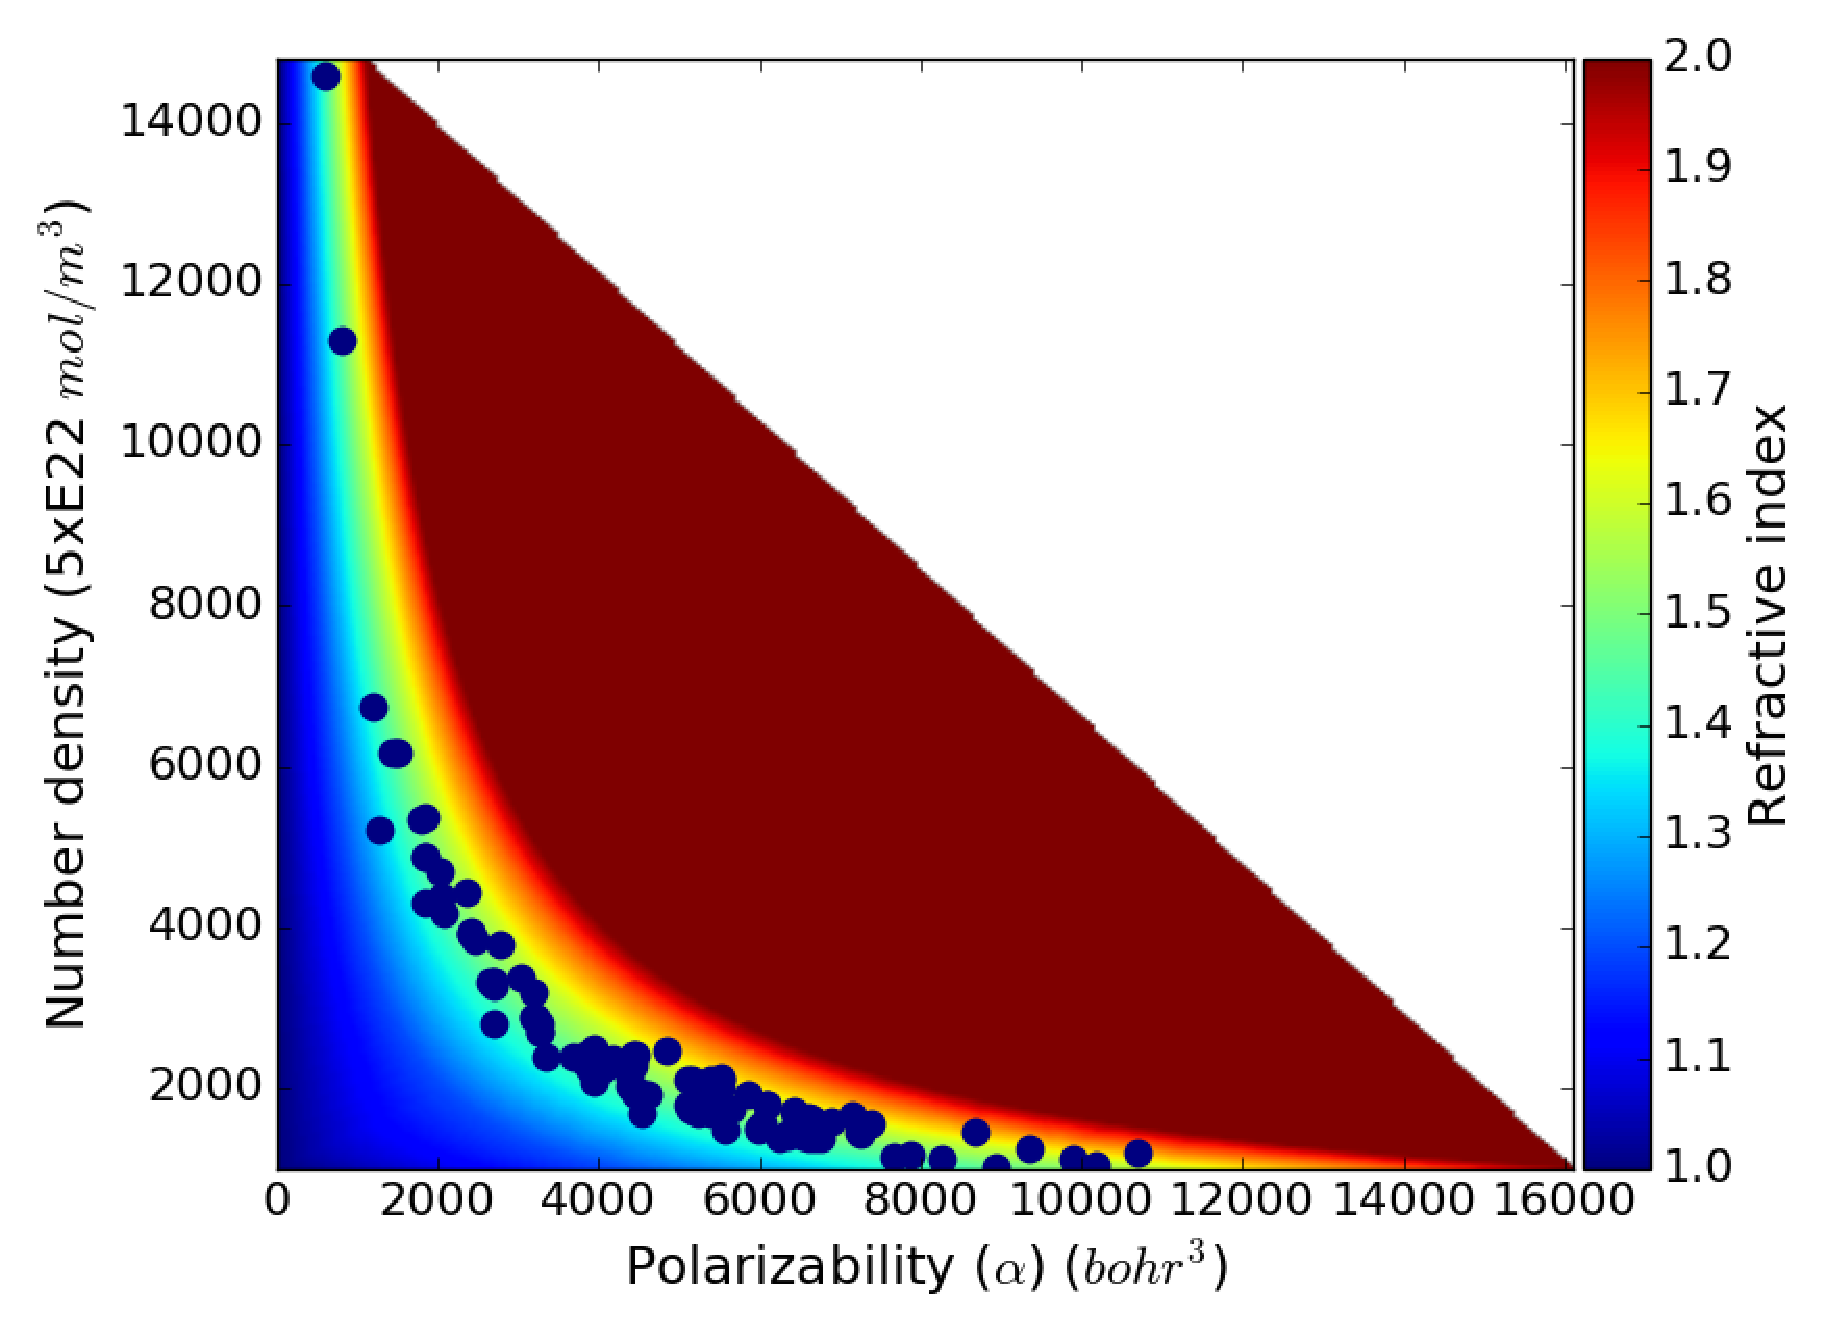
\includegraphics[width=0.744\textwidth]{Chapter-5/Figures/Den_pol_contour.eps}
	\caption{Contour plot representing the dependence of RI on the polarizability and number density. Blue dots refer to the 112 polymers used to develop RI model.} 
	\label{fig:Den_pol_contour} 
\end{figure}  

%2.	RI value of about 10 PI polymers and compare with the experimental values.

\newcolumntype{C}[1]{>{\centering\arraybackslash}m{#1}}

\begin{table}[htbp]
	\centering
	\caption{Comparison of RI values from RI prediction model with the experimental values of 10 PI candidates} \label{tab:comparison}
	\renewcommand{\arraystretch}{1.5}% Spread rows out...
	\label{Table_comp}
	\begin{tabular}{>{\centering\bfseries}m{1in}|c| >{\centering}m{1in} >{\centering}m{1in} >{\centering\arraybackslash}m{1in}}
		%\begin{tabular}{|C{1.5cm}|c|C{1.6cm}|C{1.5cm}|C{1.5cm}|}
		\multicolumn{5}{l}{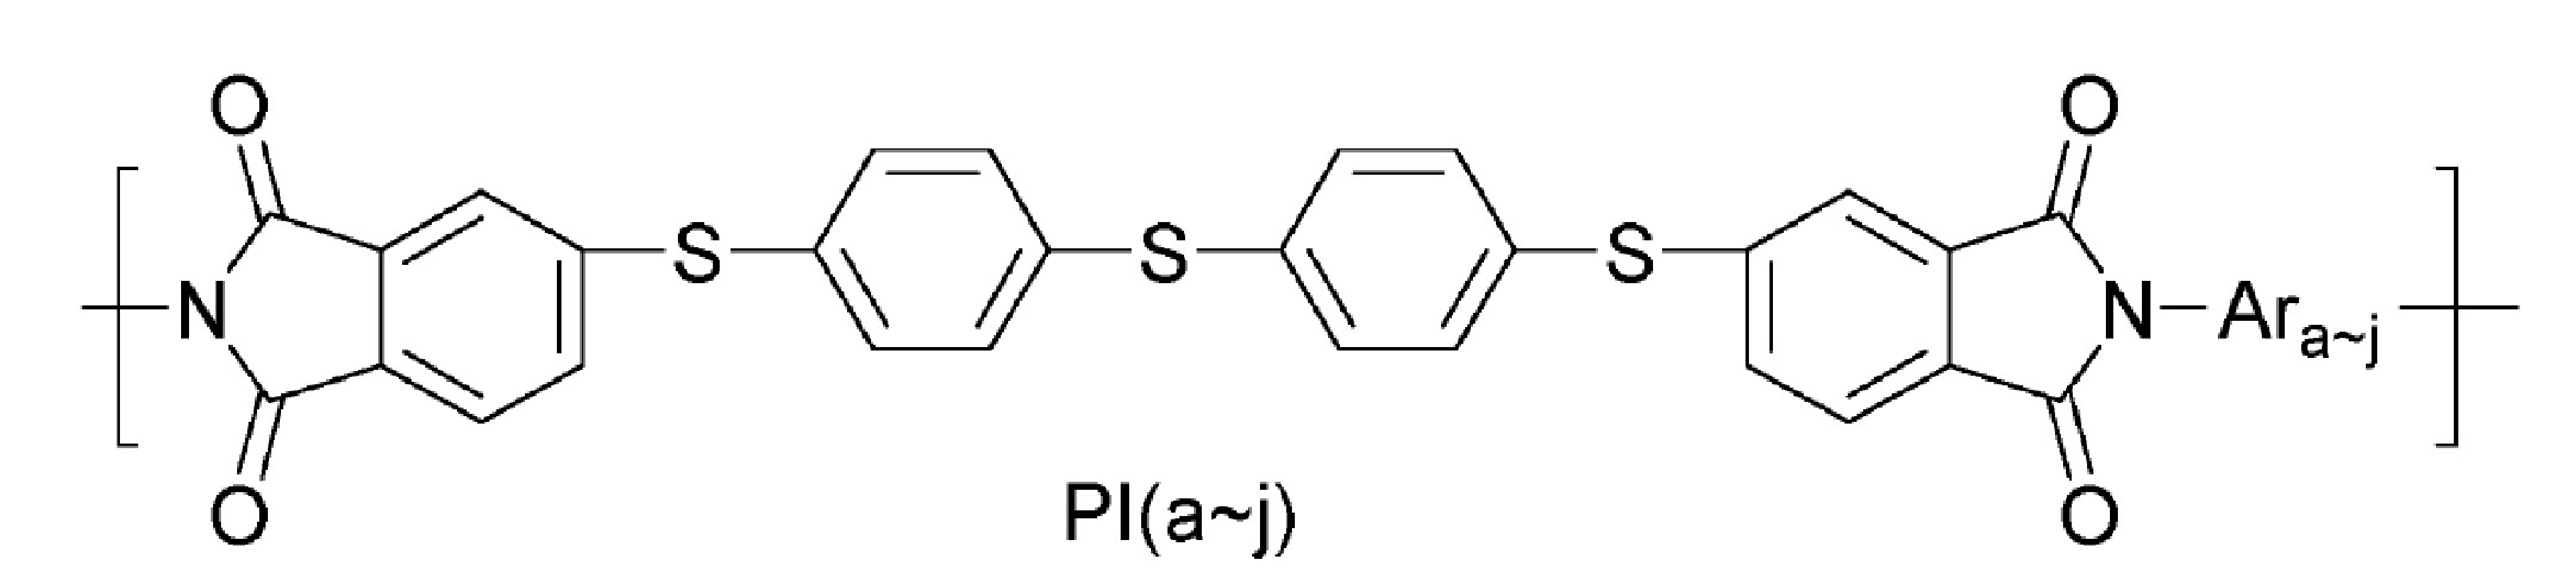
\includegraphics[width=0.5\textwidth]{Chapter-5/Figures/PI_strcutres/PI.eps}}      \\ \hline
		\multicolumn{1}{|C{1cm}|}{$\mathrm{Ar}_\mathrm{a-j}$} & \multicolumn{1}{c|}{Structure} & \multicolumn{1}{C{2.2cm}|}{Experiment value \cite{Liu2009}} & \multicolumn{1}{C{2cm}|}{Calculated value} & \multicolumn{1}{C{1.4cm}|}{Error}  \\ 
		\multicolumn{1}{|c|}{a}       & \multicolumn{1}{l|}{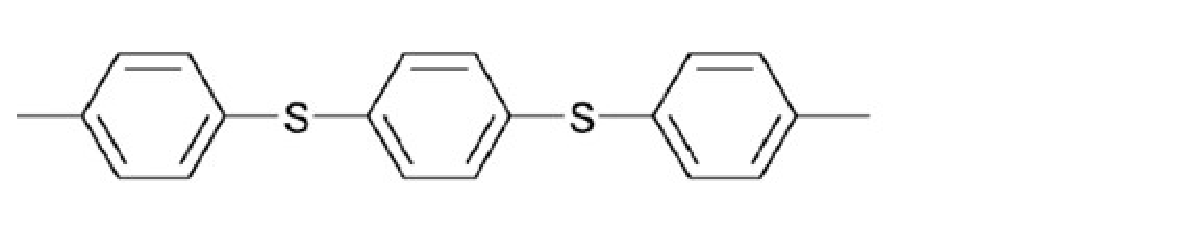
\includegraphics[width=0.4\textwidth]{Chapter-5/Figures/PI_strcutres/a.eps}}          & \multicolumn{1}{c|}{1.746}            & \multicolumn{1}{c|}{1.738}            & \multicolumn{1}{c|}{-0.008} \\ 
		\multicolumn{1}{|c|}{b}       & \multicolumn{1}{l|}{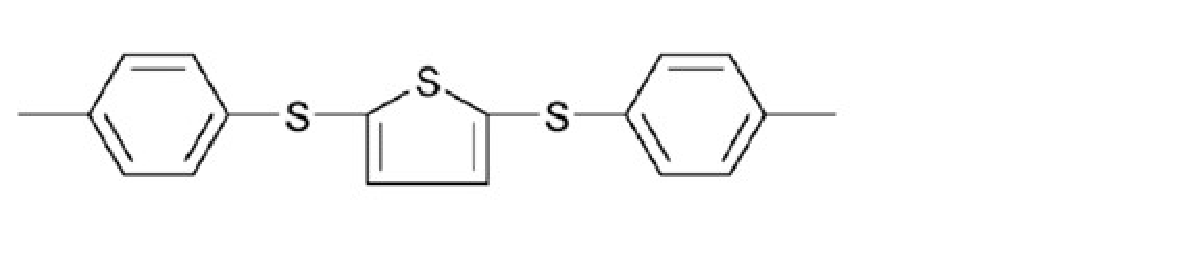
\includegraphics[width=0.4\textwidth]{Chapter-5/Figures/PI_strcutres/b.eps}}          & \multicolumn{1}{c|}{1.753}            & \multicolumn{1}{c|}{1.739}            & \multicolumn{1}{c|}{-0.013} \\ 
		\multicolumn{1}{|c|}{c}       & \multicolumn{1}{l|}{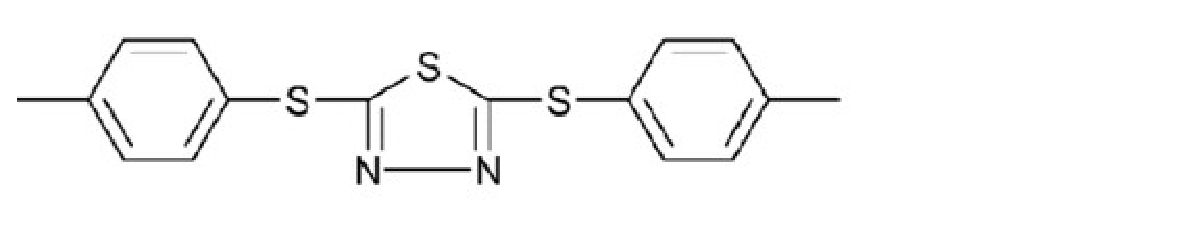
\includegraphics[width=0.4\textwidth]{Chapter-5/Figures/PI_strcutres/c.eps}}          & \multicolumn{1}{c|}{1.749}            & \multicolumn{1}{c|}{1.707}            & \multicolumn{1}{c|}{-0.042} \\ 
		\multicolumn{1}{|c|}{d}       & \multicolumn{1}{l|}{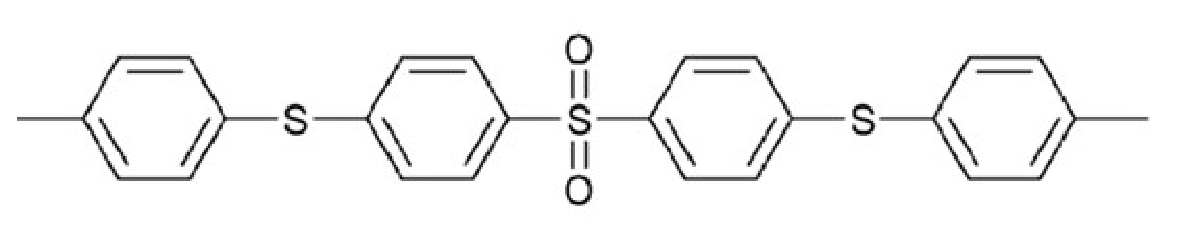
\includegraphics[width=0.4\textwidth]{Chapter-5/Figures/PI_strcutres/d.eps}}          & \multicolumn{1}{c|}{1.748}            & \multicolumn{1}{c|}{1.751}            & \multicolumn{1}{c|}{0.003}  \\ 
		\multicolumn{1}{|c|}{e}       & \multicolumn{1}{l|}{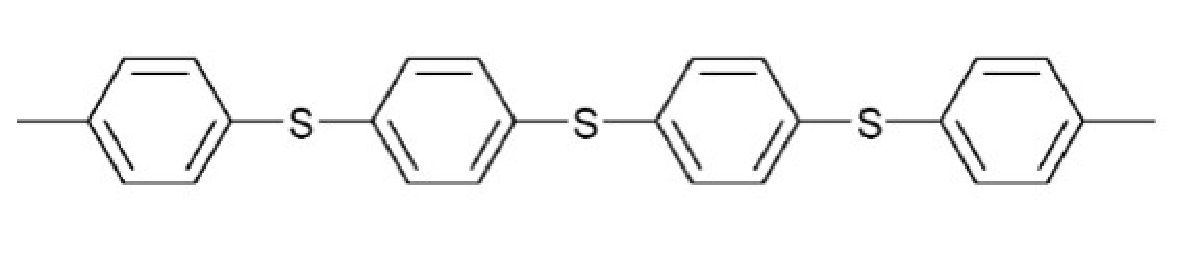
\includegraphics[width=0.4\textwidth]{Chapter-5/Figures/PI_strcutres/e.eps}}          & \multicolumn{1}{c|}{1.733}            & \multicolumn{1}{c|}{1.760}            & \multicolumn{1}{c|}{0.027}  \\ 
		\multicolumn{1}{|c|}{f}       & \multicolumn{1}{l|}{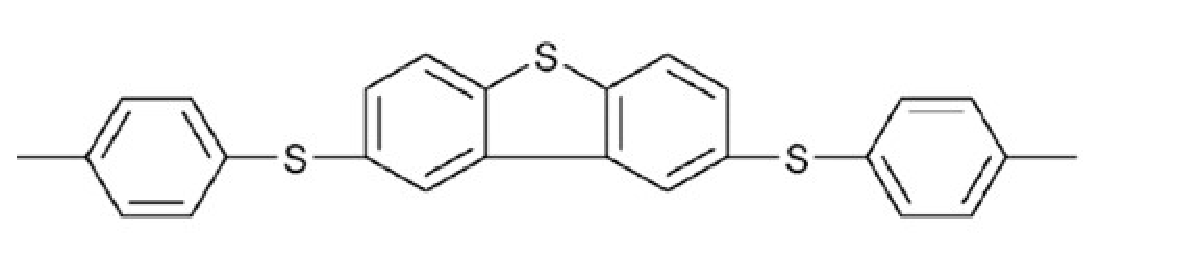
\includegraphics[width=0.4\textwidth]{Chapter-5/Figures/PI_strcutres/f.eps}}          & \multicolumn{1}{c|}{1.758}            & \multicolumn{1}{c|}{1.779}            & \multicolumn{1}{c|}{0.021}  \\ 
		\multicolumn{1}{|c|}{g}       & \multicolumn{1}{l|}{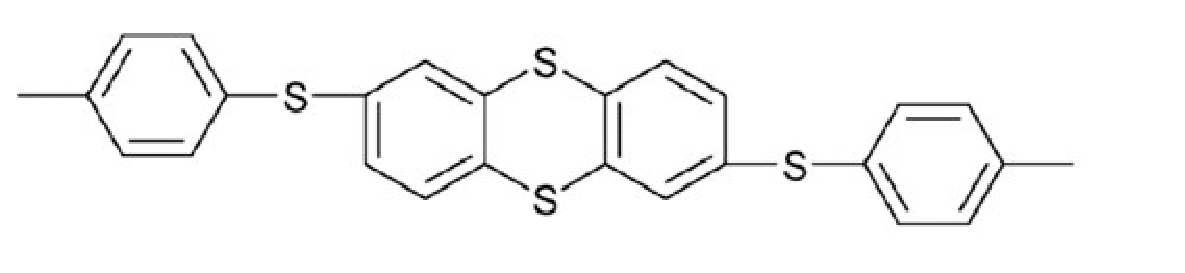
\includegraphics[width=0.4\textwidth]{Chapter-5/Figures/PI_strcutres/g.eps}}          & \multicolumn{1}{c|}{1.760}            & \multicolumn{1}{c|}{1.735}            & \multicolumn{1}{c|}{-0.025} \\ 
		\multicolumn{1}{|c|}{h}       & \multicolumn{1}{l|}{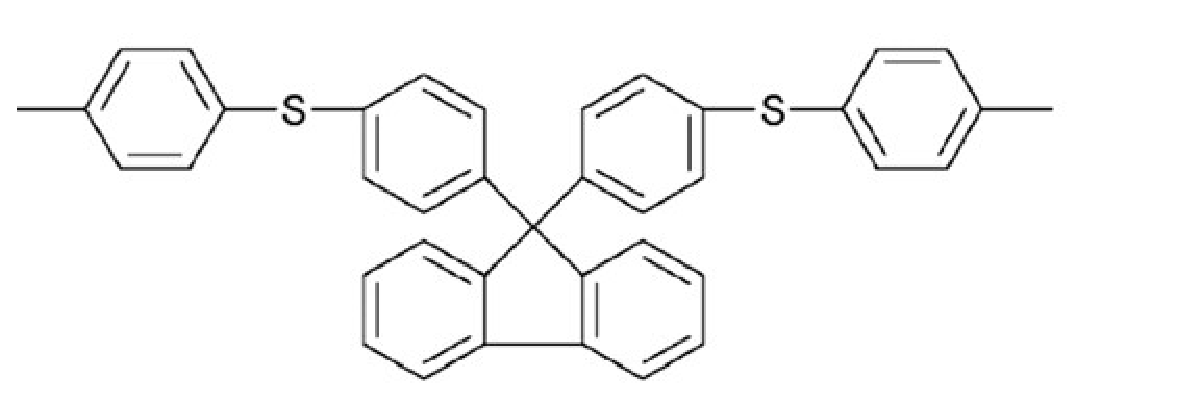
\includegraphics[width=0.4\textwidth]{Chapter-5/Figures/PI_strcutres/h.eps}}          & \multicolumn{1}{c|}{1.726}            & \multicolumn{1}{c|}{1.741}            & \multicolumn{1}{c|}{0.015}  \\ 
		\multicolumn{1}{|c|}{i}       & \multicolumn{1}{l|}{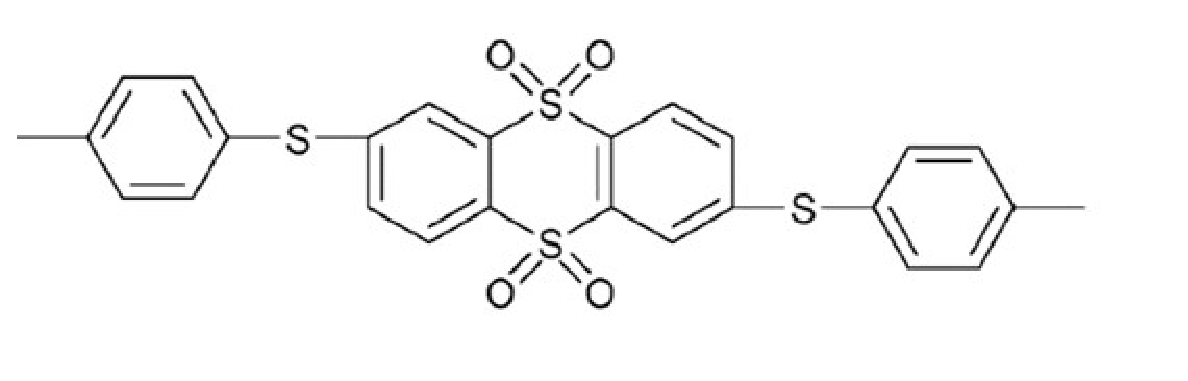
\includegraphics[width=0.4\textwidth]{Chapter-5/Figures/PI_strcutres/i.eps}}          & \multicolumn{1}{c|}{1.737}            & \multicolumn{1}{c|}{1.743}            & \multicolumn{1}{c|}{0.005}  \\ 
		\multicolumn{1}{|c|}{j}       & \multicolumn{1}{l|}{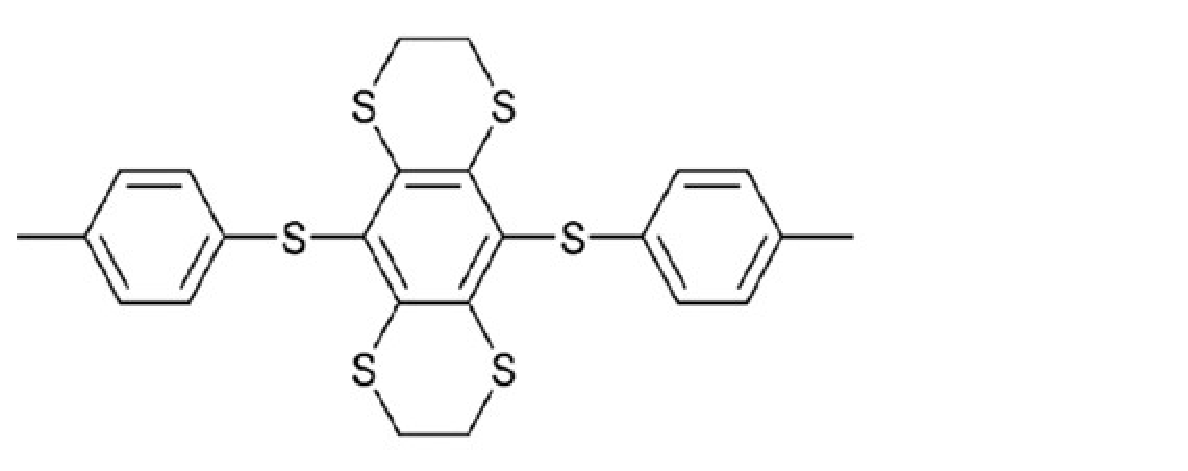
\includegraphics[width=0.4\textwidth]{Chapter-5/Figures/PI_strcutres/j.eps}}          & \multicolumn{1}{c|}{1.769}            & \multicolumn{1}{c|}{1.724}            & \multicolumn{1}{c|}{-0.045} \\ \hline
	\end{tabular}
\end{table}

As mentioned in the methods section, we calculate the RI of PIs using a model that involves the calculation of the polarizability and the number density values. We previously tested this model against 112 non-conjugated polymers, however, there were no PI candidates in this list. Therefore, to check the validity of our RI model on the PI structures, we compared the model with experimental RI values of 10 PIs shown in table \ref{Table_comp}. The RMSD of the model is 0.024, suggesting that our model is accurate for calculating the RI of PIs.

%3.	Explanation of the selection of building blocks and the process of creation of PI library. PI split into two segments, $R_1$ and $R_2$, and separately studied. X number of $R_1$ and Y number of $R_2$ were created based on generation rules. 
In search of high RI PIs, we created about 50 thousand and 220 thousand structures of $R_1$ and $R_2$, respectively, using 29 promising building blocks as shown in Fig. \ref{fig:Building_blocks}. Combining all these $R_1$ and $R_2$ structures to form PI could lead to a total of 11 billion PIs. However, virtual high-throughput screening of such an astronomical number of structures is not a viable option. Therefore, we narrowed down the number of possible PI candidates by picking the best of the $R_1$ and $R_2$ structures. We did so by computing the RI values of the individual $R_1$ and $R_2$ structures. After the screening of these structures, we developed the most promising PI candidates by combining the top $R_1$ and $R_2$ structure as shown in \ref{fig:Building_blocks}. 
%TODO - unclear, need a better explanation.

%4.	The RI values of the $R_1$ and $R_2$ library and the top candidates. The histogram of $R_2$.
In this paper, we discuss the results of $R_2$ structures. Figure \ref{fig:RI_hist} shows the RI distribution of $R_2$ structures. We observe a Gaussian type distribution for the RI values of $R_2$ structures. Most of the candidates have RI values between 1.5 and 1.7, which suggests that there is a strong possibility of obtaining molecules with such RI values using empirical approaches. However, using a computational approach, we we were able to find the outliers, i.e., the candidates with RI values greater than 1.7. 
%Using the developed RI prediction protocol and casting this protocol into the ChemHTPS framework, the most promising candidates for $R_1$ and $R_2$ structures were identified. 

\begin{figure}[htbp] 
	\centering
	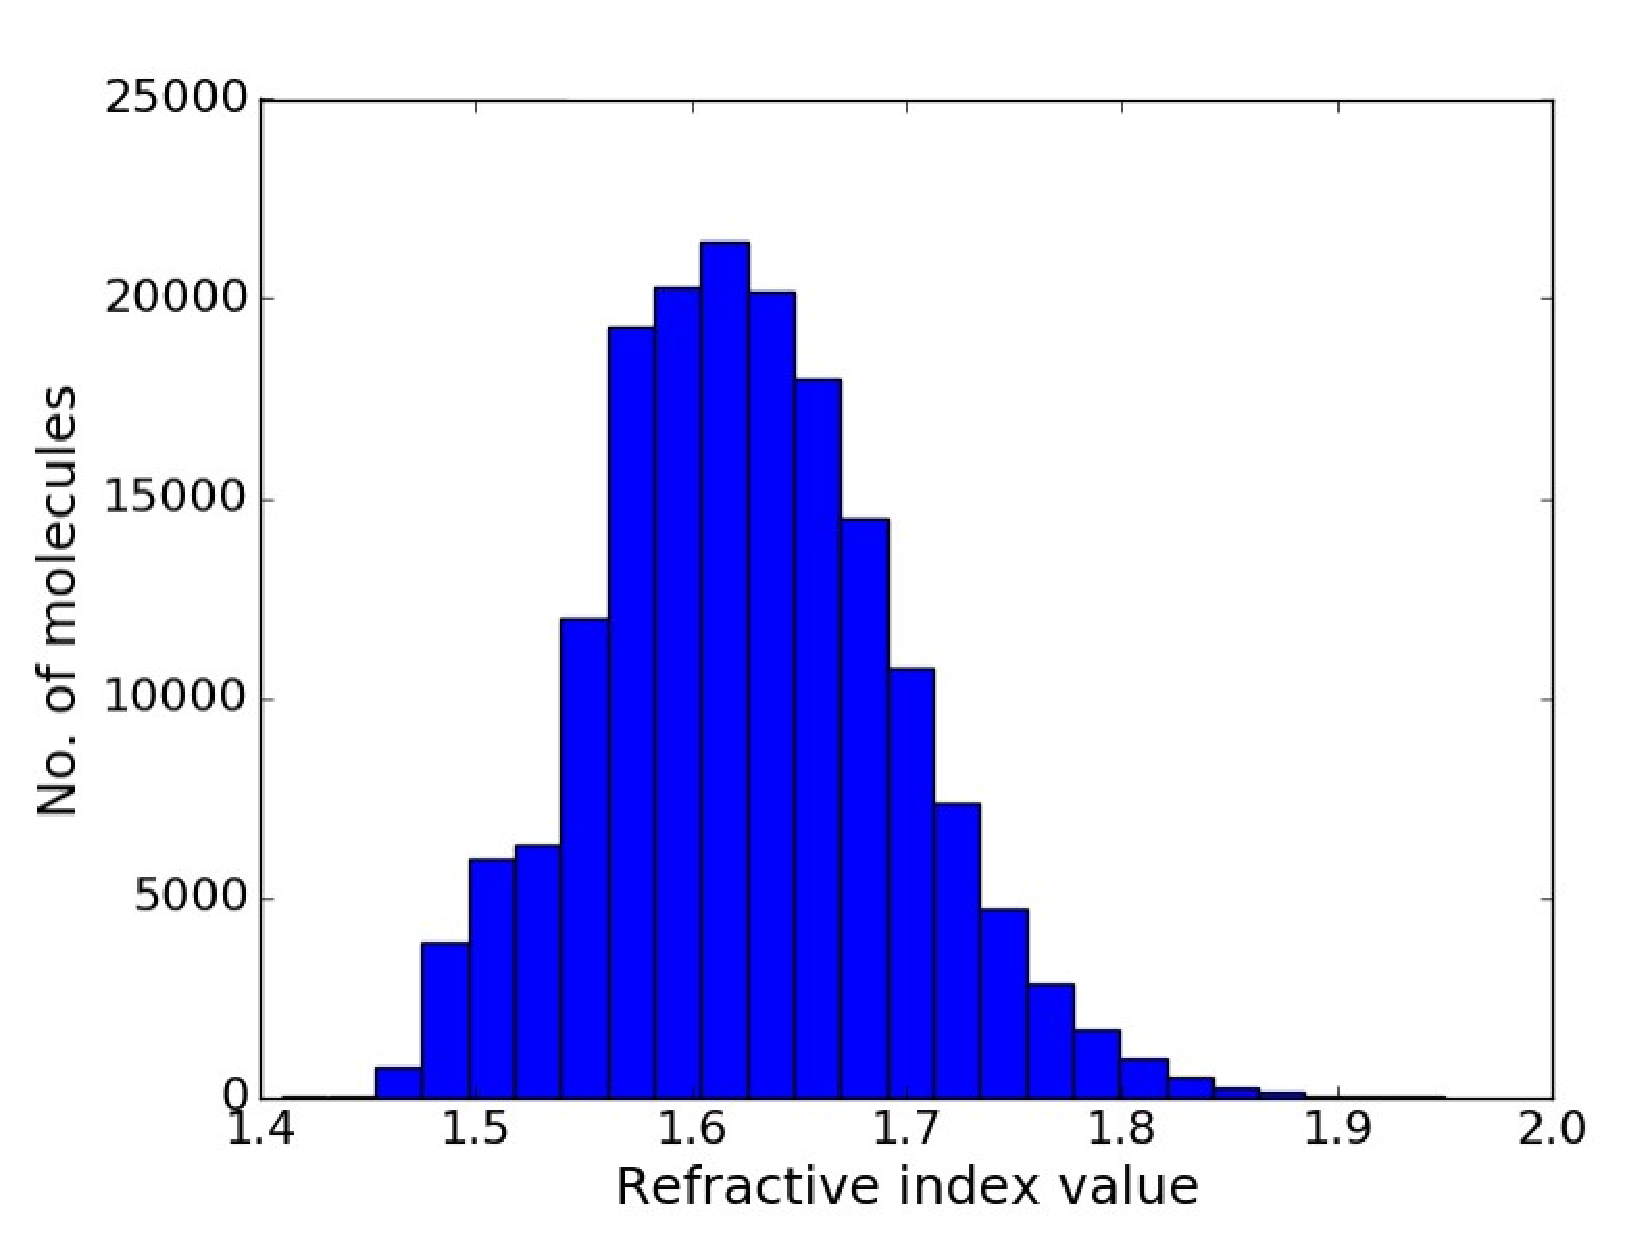
\includegraphics[width=0.700\textwidth]{Chapter-5/Figures/RI_histogram.eps}
	\caption{RI distribution of the $R_2$ structures} 
	\label{fig:RI_hist} 
\end{figure}  

%5.	Combining the best of $R_1$ and $R_2$ to form a full PI.
The top 100 structures of $R_1$ type and top 1000 structures of $R_2$ type are selected to form 100,000 PI monomers. We casted these PI structures into our HTPS framework to evaluate the RI values.
%TODO - need more information here.

%6.	Looking at the building blocks contribution
\begin{figure}[htbp] 
	\centering
	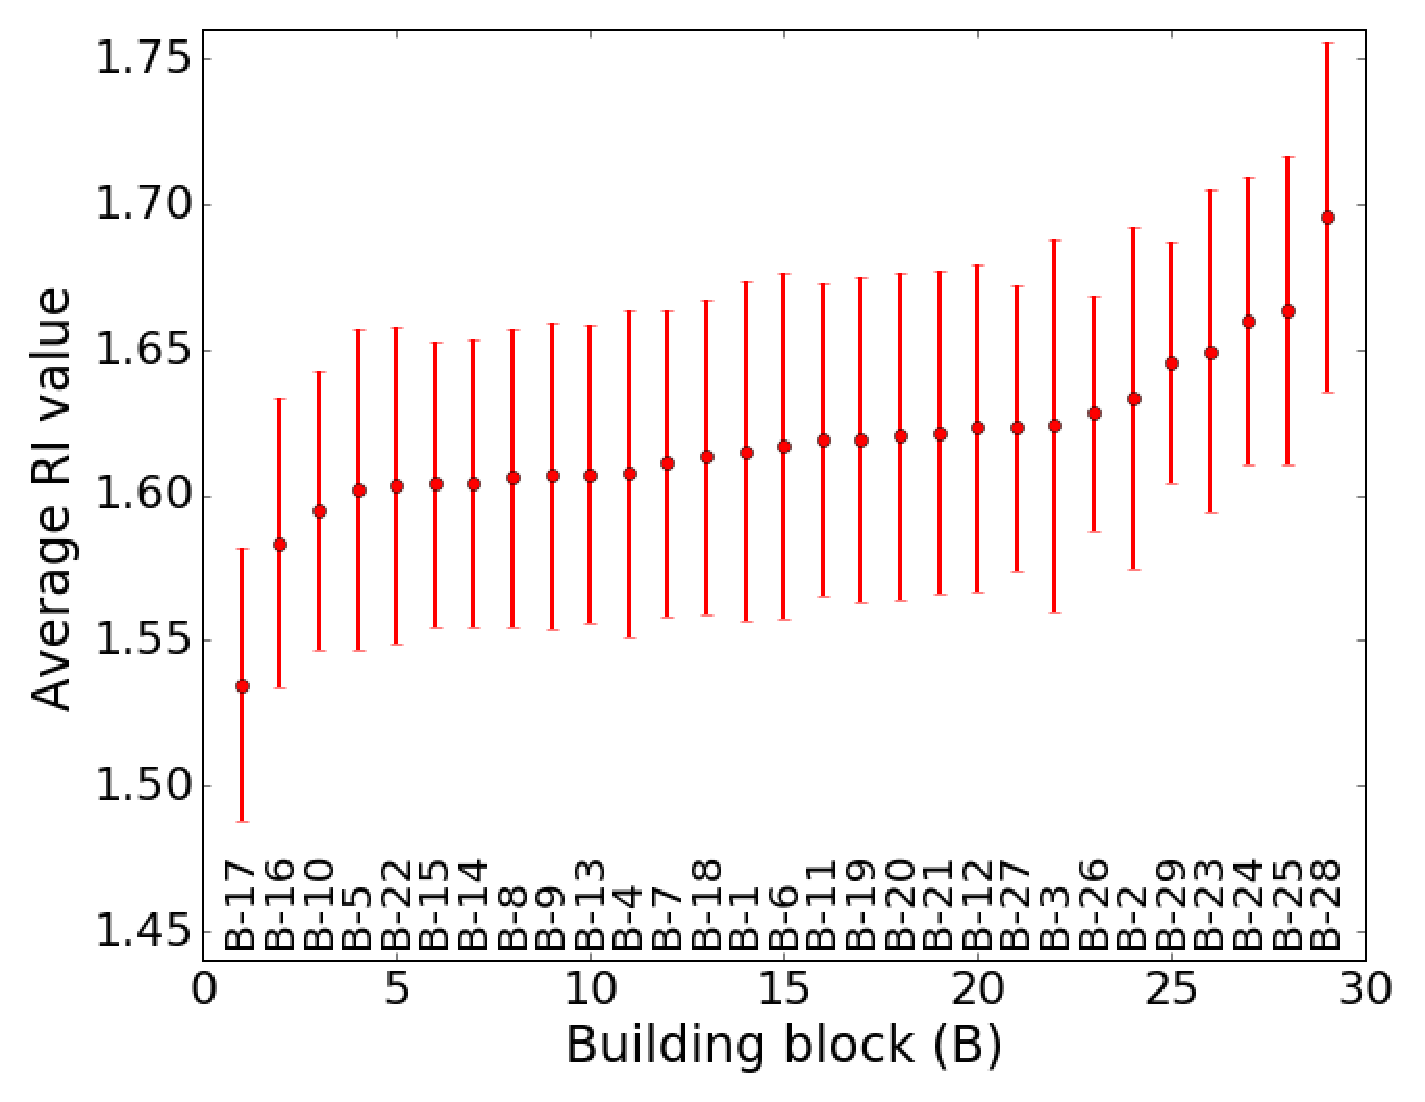
\includegraphics[width=0.700\textwidth]{Chapter-5/Figures/BB_avg_RI.eps}
	\caption{Average RI of the structures containing each building block in the top 10\% candidates of $R_2$. } 
	\label{fig:BB_avg_RI} 
\end{figure}  

\begin{figure}[htbp] 
	\centering
	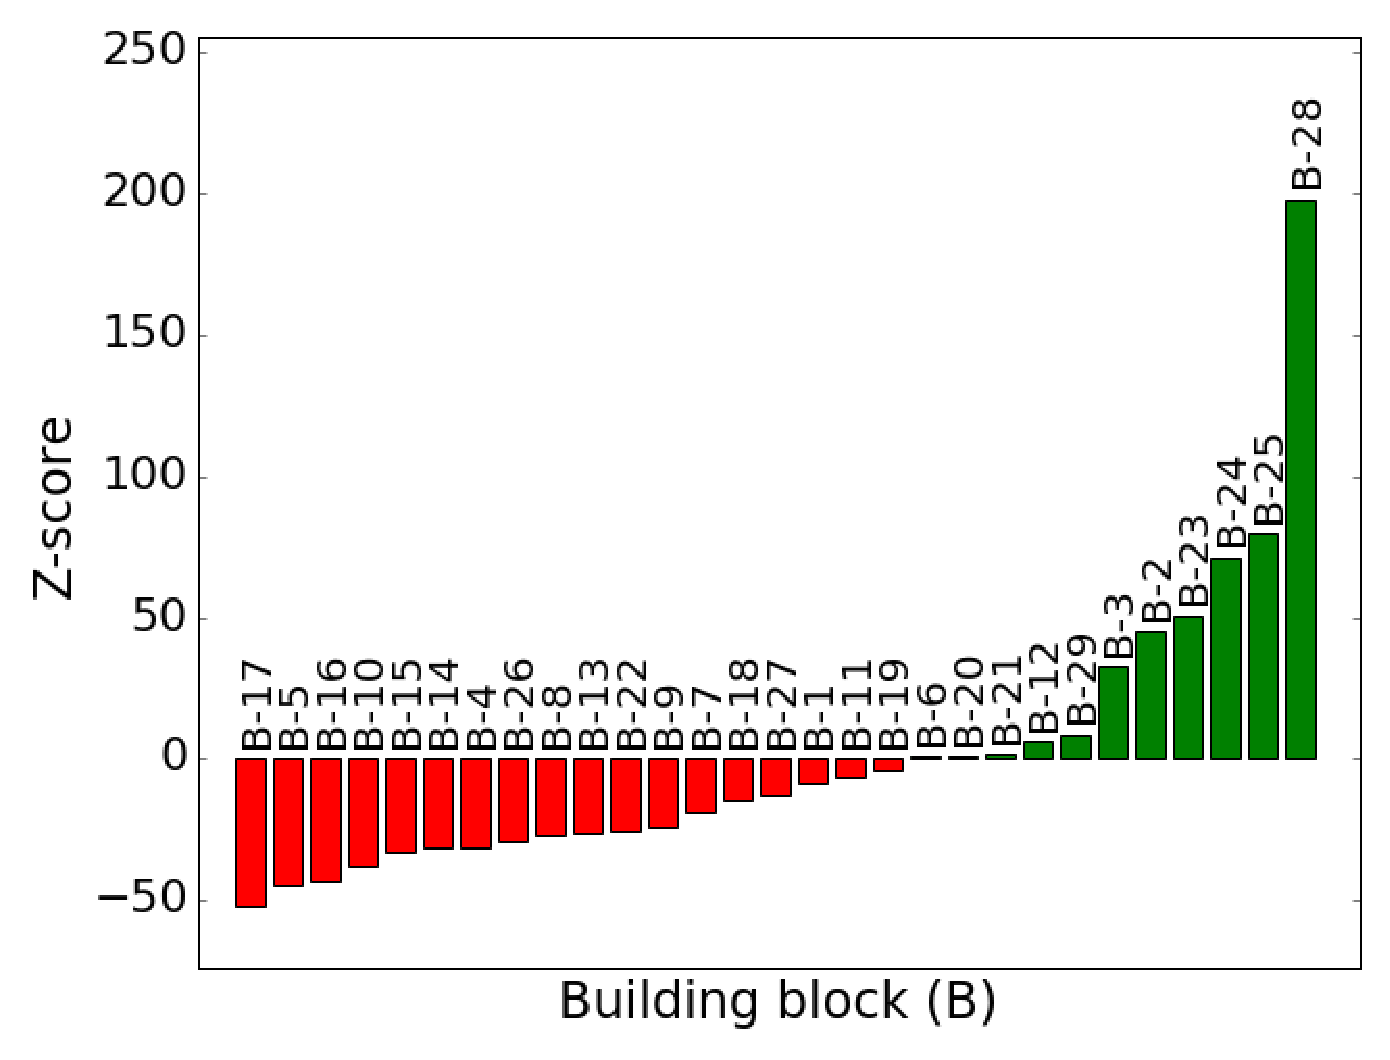
\includegraphics[width=0.700\textwidth]{Chapter-5/Figures/BB_top_Z.eps}
	\caption{Z-score of each building block in the top 10\% candidates of $R_2$.} 
	\label{fig:BB_top_Z} 
\end{figure}  

Besides identifying the potential HRIP candidates, understanding the underlying structure-property relationships would enable us to discern candidates with optimal RI values. This would help us create a special subset of candidates for our experimental collaborators to further explore. To do so, we tried to recognize the contribution of each building block towards a targeted property to aid in identifying favorable synergies in building block combinations, with an aim to narrow our chemical search space. We decided to implement this into our studies by looking at two different scoring systems for the building blocks: i) the average RI value of the candidates which contain each building block and ii) the Z-score of each building block in the top candidates. We plotted the results obtained from the first method in Fig. \ref{fig:BB_avg_RI}, which presents the RI distribution of candidates containing a particular building block. Here, we found that for the $R_2$ structures, candidates containing building blocks 24, 25 and 28 have the highest RI values, while the candidates containing building blocks 17, 16 and 10 showed the lowest RI values. Figure \ref{fig:BB_top_Z} on the other hand shows the z-scores. This technique is favored as a higher z-score would mean a larger prevalence of a particular building block in a HRIP. In our case, we picked the top 10\% of candidates in terms of their RI values and evaluated the Z-scores of individual building blocks in this subset. The green color in the Fig. \ref{fig:BB_top_Z} represents a positive Z-score, whereas the red color represents a negative Z-score. This technique confirmed our results obtained by the first method as the Z-score values also suggest that the building blocks 24, 25 and 28 are the most promising for developing HRIPs.  

\begin{figure*}[htbp] 
	\centering
	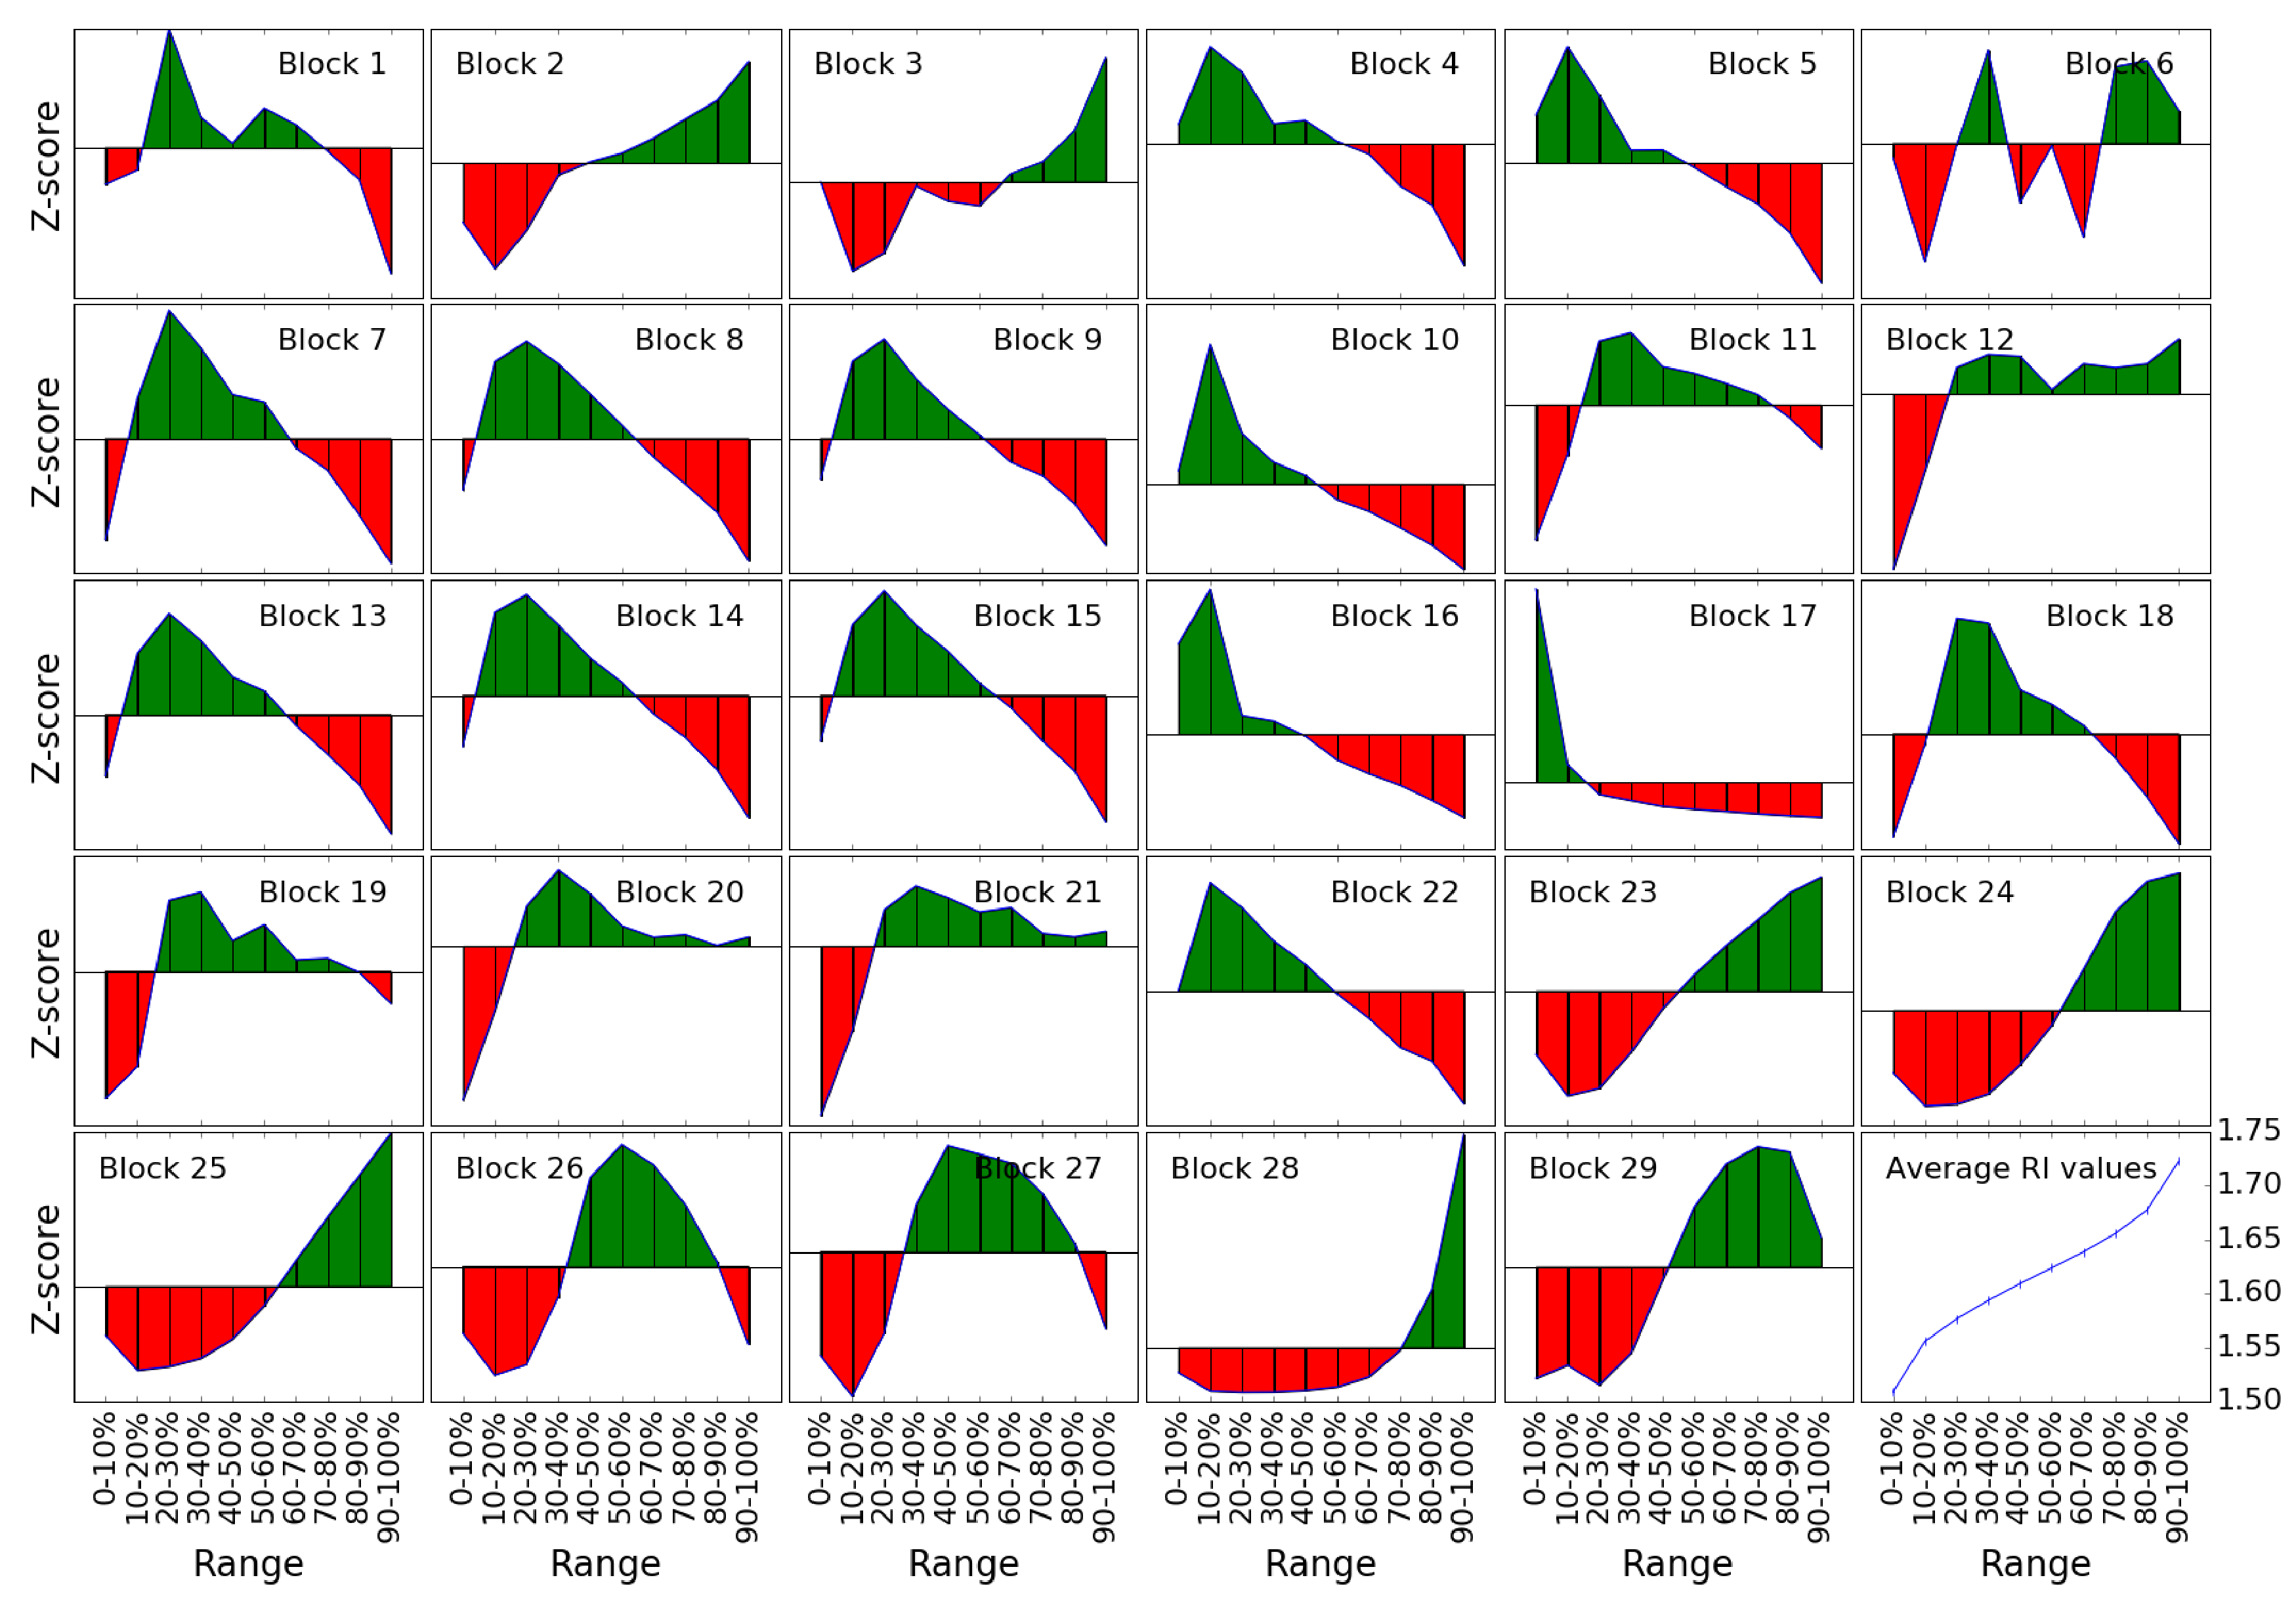
\includegraphics[width=1.00\textwidth]{Chapter-5/Figures/All_BB_Z.eps}
	\caption{Z-score of each building block in all the $R_2$ structures. } 
	\label{fig:All_BB_Z} 
\end{figure*}  

The above Z-score analysis only gives the prevalence of building blocks in the top 10\% candidates, but not the remaining ones. In order to generate a more comprehensive structure-property relationship, we evaluated the Z-score of building blocks in the full spectrum of the library. For this, the library was divided into 10 subsets ordered by increasing RI values. We evaluated the Z-score of the building blocks in each of these 10 subsets and plotted them with increasing RI values (see Fig. \ref{fig:All_BB_Z}). The green color represents a positive Z-score and the red represents a negative Z-score. We observed certain trends in this plot:
\begin{enumerate}
	\item The Z-score of building blocks 2, 3, 23, 24, 25, 28 and 29 increase with increasing RI values.
	\item The Z-score of building blocks 4, 5, 10, 16, 17 and 22 decreases with increasing RI values.
	\item The Z-score of building blocks 7, 8, 9, 11, 13, 14, 15, 18, 26 and 27 change from a negative value to a positive value before becoming negative again.
	\item The building blocks 1, 6, 12,19, 20 and 21 do not show a clear trend, therefore appear to have less impact on the RI values 
\end{enumerate}

%#Using such analysis we could identify building blocks whose presence lead to a higher RI value. 

\begin{figure*}[htbp] 
	\centering
	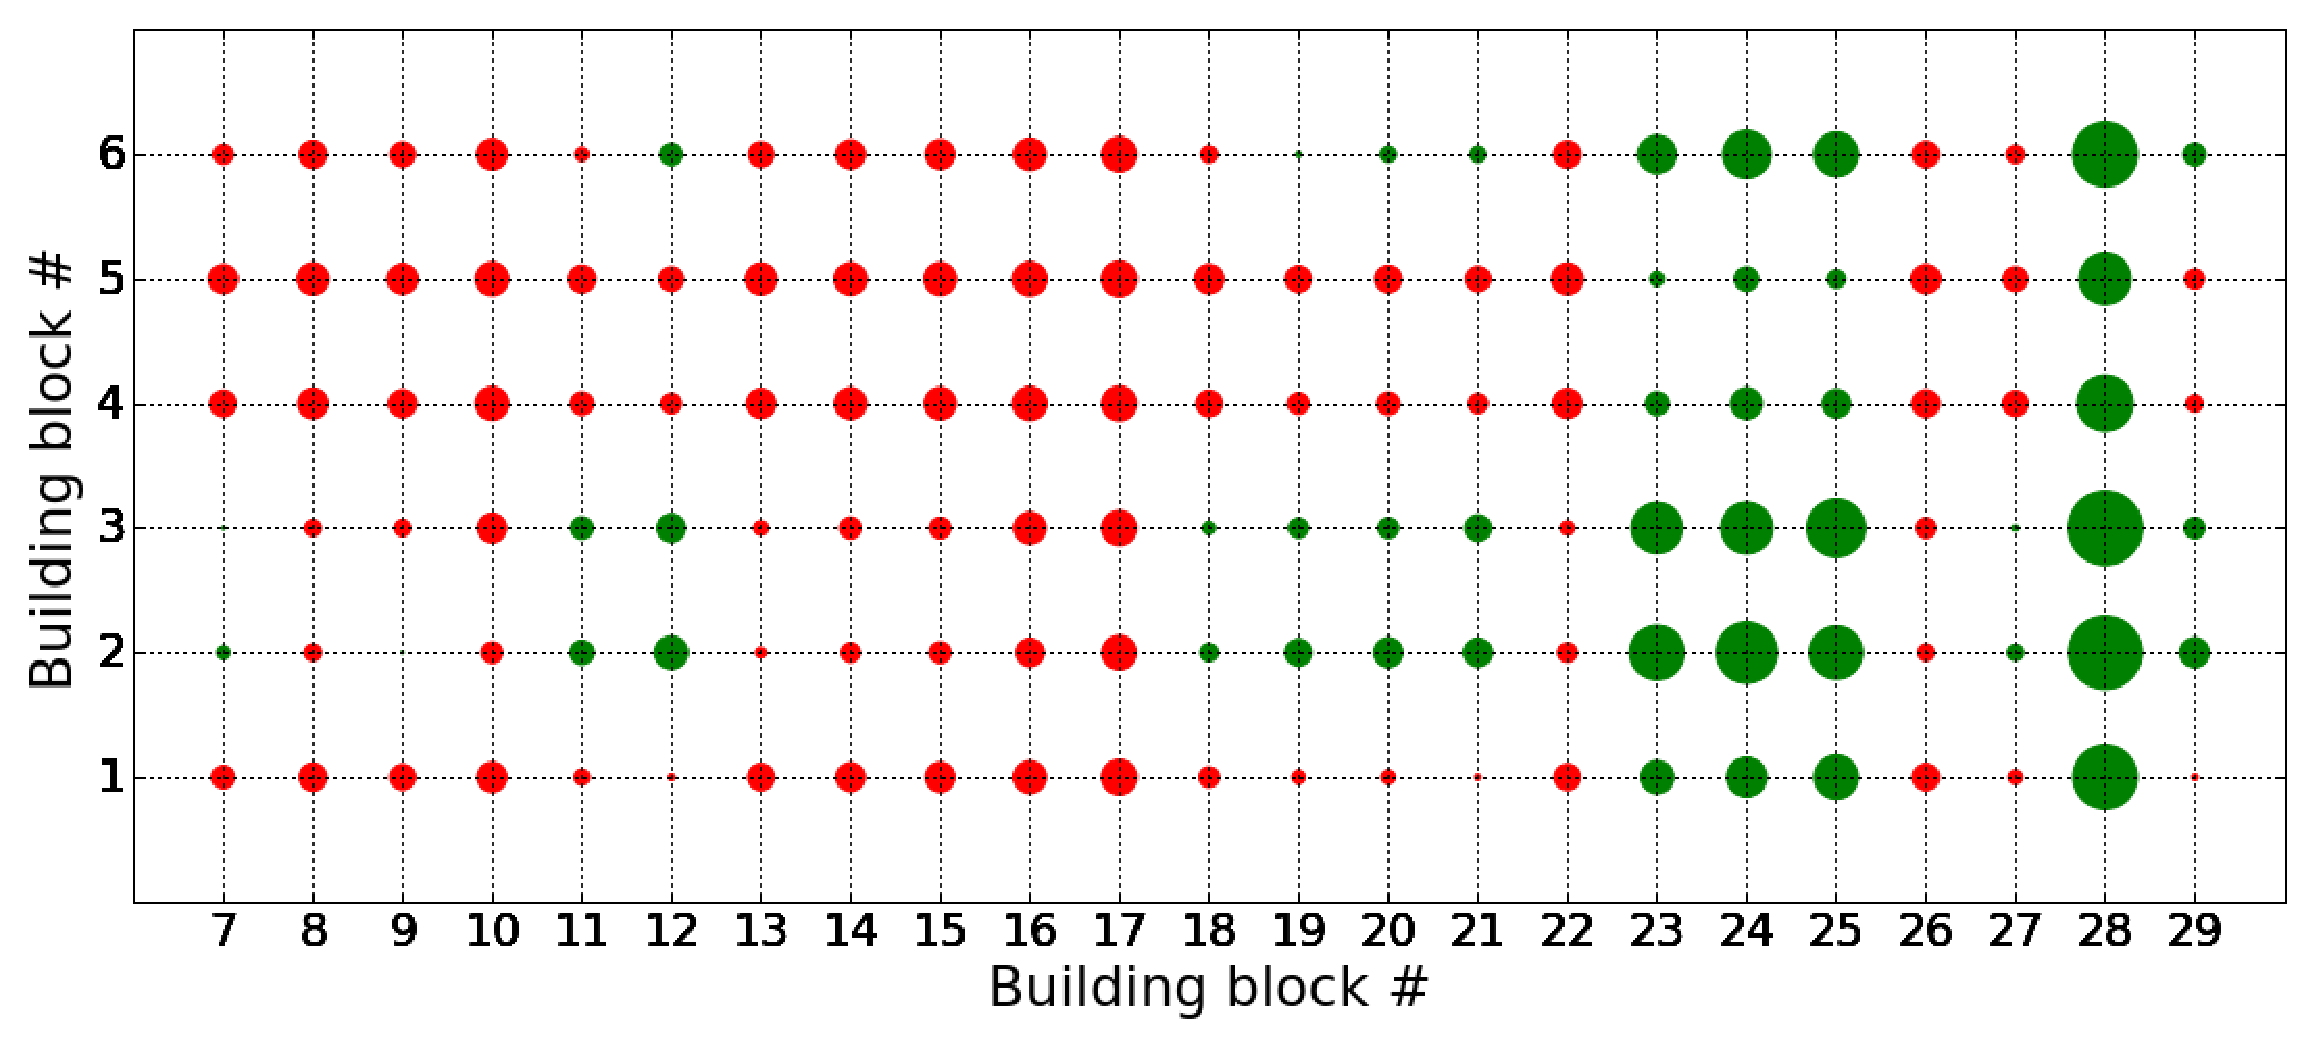
\includegraphics[width=1.00\textwidth]{Chapter-5/Figures/Bonds_top_Z.eps}
	\caption{Z-score of building block combinations in the top 10\% candidates of $R_2$.} 
	\label{fig:Bonds_top_Z} 
\end{figure*}  

In addition to building blocks contribution to RI values, it is also important to note the impact of various building block combinations to further understand the structure-property relationship. Therefore, we calculated the Z-scores of all the possible building block combinations in the top candidates. Fig. \ref{fig:Bonds_top_Z} illustrates which building blocks combinations are promising for high RI polymers. The size of the circle in the plot represents the magnitude of the Z-score value. The green color of the circle indicates a positive Z-score, whereas the red circle indicates a negative value. Using this figure, we can see that the combination of building block 28 with blocks 2 and 3 occur very frequently in top candidates given by the large size of the circle. The combinations of building blocks 23, 24, 25 and 28 with building blocks 1, 2 and 3 appear to be promising for the creating HRIPs. 
%TODO - further discussion required

The above structure-property relationships demonstrate the best building blocks and the combinations of these building blocks which are highly promising in developing HRIPs. We will use these guiding principles to create the next generation of HRIPs, and further validate these candidates by synthesizing them and testing their RI values. The best candidates from this study are currently being synthesized by our experimental collaborators, which we will be publishing soon.
%TODO - check with Prof Cheng regarding the results. 

\section{Conclusions}
\label{sec:conclusions5}

We demonstrated the developed RI model is successful in calculating the RI values of polyimides. We successfully created a molecular library of 270,000 PIs from promising building blocks, suggested by our experimental collaborators. We identified the best candidates by screening the library using our virtual high-throughput screening framework. The screening study resulted in more than 2000 PIs with RI values greater than 1.8. In addition to identifying high RI candidates, we applied materials informatics and data mining techniques to understand the relationship between the molecular structure and the RI values. Using these techniques, we identified building blocks and combinations of building blocks that are prominent in the top RI candidates. The developed rational design framework is successful for the accelerated discovery of polyimides with exceptional RI values.


